\chapter{Quantum Monte Carlo Methods} \label{chp:methods}
%\epigraph{Great quote.}{Author}
\begin{figure}[H]
	\centering
	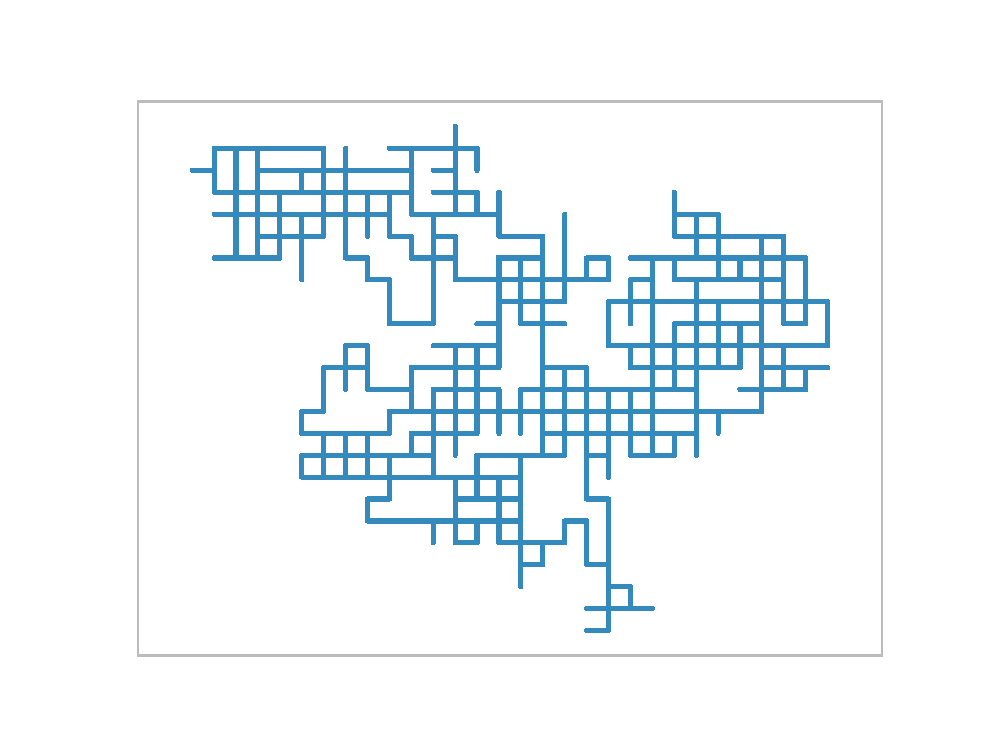
\includegraphics[scale=0.6]{../Images/randomwalk.eps}
	\caption{Random walker on a two-dimensional grid, 1000 moves.}
\end{figure}

Quantum Monte Carlo methods (QMC) represent a variety \textit{ab initio} methods that attempt to solve the Schrödinger equation using stochastic Monte Carlo integration. \textit{Ab initio} reads "from first principles", which implies that the methods constitute a fundamental approach to the problem. They all seek to evaluate the multi-dimensional integrals that represent various quantum mechanical expectation values. The expression for the energy reads
\begin{empheq}[box={\mybluebox[5pt]}]{equation}
E_0= \mel{\Psi_0}{\hat{\mathcal{H}}}{\Psi_0}= \frac{\int d\bs{X}\Psi_0(\bs{X})^*\hat{\mathcal{H}}\Psi_0(\bs{X})}{\int d\bs{X}\Psi_0(\bs{X})^*\Psi_0(\bs{X})},
\label{eq:schrodingergroundstate}
\end{empheq}
which provides the ground state energy expectation value for the exact ground state wave function $\Psi_0(\bs{X})$ with $\bs{X}=\{\{\bs{r}_1,\sigma_1\},\{\bs{r}_2,\sigma_2\},\hdots,\{\bs{r}_N,\sigma_N\}\}$ as the collective coordinates of the $N$ particles. As aforementioned, this integral is analytically infeasible for more or less all interesting systems, evokes the need for numerical methods like QMC. As we will stick to ground state calculations, the wave function $\Psi(\bs{X})$ implies the many-body ground state wave function from this point.

In Monte Carlo integration, we use random numbers to evaluate integrals numerically. Typically, we want to estimate an expectation value $\langle\hat{O}\rangle$ by approximating the integral with the sum,
\begin{equation}
\langle \hat{O}\rangle\equiv\int_{-\infty}^{\infty}d\bs{x}P(\bs{x})\hat{O}(\bs{x})\approx\frac{1}{M}\sum_{i=1}^M\hat{O}(\bs{x}_i),
\label{eq:montecarlointegration}
\end{equation}
where $M$ is the number of \textit{Monte Carlo cycles} and the coordinates $\bs{x}_i$ are drawn randomly from the probability density function $P(\bs{x})$. A great advantage of the QMC methods, is that we obtain approximative ground state wave functions when solving equation \eqref{eq:schrodingergroundstate}, which by the fourth postulate of quantum mechanics allows estimations of the ground state expectation values associated with other operators as well. 

Two widely used QMC methods are the variational Monte Carlo method (VMC) and the diffusion Monte Carlo method (DMC), where the former is arguably the simplest of all the QMC methods. It attempts to solve the integrals in equation \eqref{eq:schrodingergroundstate} directly by varying parameters, with the support of the variational principle presented in section \ref{sec:variationalprinciple}. This makes VMC a comparably computationally cheap method, but the performance is usually not in the league of the best methods. Diffusion Monte Carlo, on the other hand, is computationally expensive, but is also potentially numerically exact, making it a preferred method when high accuracy is needed. At first glance, it might seems like a tradeoff where VMC is used when computational time is more important than the accuracy and DMC is used when the opposite is true. However, DMC requires a wave function input which is close to the exact wave function, forcing us first to run a VMC calculation to obtain this wave function before the DMC machinery can be started.

As VMC is our main focus in this work, it will be explained thoroughly in this chapter. After that, we will briefly explain the idea behind the DMC method, but since this method is not implemented, it will not be our main priority. To reveal the uncertainty of our results, we will also discuss some methods to estimate the errors, in particular, the blocking method.

\section{Variational Monte Carlo} \label{sec:vmc}
The variational Monte Carlo method (hereafter the VMC method) is today widely used when it comes to the study of ground state properties of quantum many-body systems. It makes use of Markov chain Monte Carlo methods, often abbreviated MCMC, where the particles are assumed to be moving in Markov chains controlled by Monte Carlo simulations. Going back to the variational principle in equation \eqref{eq:variationalprinciple}, one observes that by choosing an approved wave function, one gets an energy larger or equal to the ground state energy.

Before we present the mathematical framework of the method, we will restate the two big challenges in many-body physics, mentioned in the introduction:
\begin{enumerate}
	\item The correct many-body wave function is generally unavailable.
	\item The many-body energy expectation value is analytically infeasible for most systems.
\end{enumerate}
In this section, we will look at how the VMC method tackles these challenges. We start with discussing the trial wave function, and set up our trial wave function ansatz. Then, we define the local energy and explain how it is used to solve the energy integral using Monte Carlo integration. In the end, we will mention some common extensions to the VMC method. 

\subsection{The trial wave function} \label{sec:trial}
The trial wave function was mentioned in section \ref{sec:cusp}, but what is actually the trial wave function? In VMC, we start from a wave function ansatz, which is our ground state wave function guess. This function is equipped with variational parameters, and in order to estimate the wave function accurately, the trial wave function needs to be able to approach the correct wave function as we vary the parameters. However, as the many-body wave function is NP-hard to calculate \supercite{troyer_computational_2005}, we will only be able to approximate it and for that reason the wave function is by many considered as the root of all evil in many-body physics. For fermionic systems, the standard trial wave function used in VMC, given a set of variational parameters $\bs{\theta}$, is the Slater-Jastrow wave function, 
\begin{empheq}[box={\mybluebox[5pt]}]{equation}
\Psi_T(\bs{X};\bs{\theta})=|\hat{S}(\bs{X};\bs{\theta})|J(\bs{X};\bs{\theta}),
\end{empheq}
where $|\hat{S}(\bs{X};\bs{\theta})|$ is a Slater determinant used to bake in the anti-symmetry discussed in section \ref{sec:symmetry} and $J(\bs{R};\bs{\theta})$ is a Jastrow factor used to model the electron-electron correlations. Recall that the general Slater determinant has the form
\begin{equation}
|\hat{S}(\bs{X};\bs{\theta})|=\frac{1}{\sqrt{N!}}
\begin{vmatrix}
\psi_1(\boldsymbol{r}_1,\sigma_1;\bs{\theta}) & \psi_2(\boldsymbol{r}_1,\sigma_1;\bs{\theta}) & \hdots & \psi_N(\boldsymbol{r}_1,\sigma_1;\bs{\theta})\\
\psi_1(\boldsymbol{r}_2,\sigma_2;\bs{\theta}) & \psi_2(\boldsymbol{r}_2,\sigma_2;\bs{\theta}) & \hdots & \psi_N(\boldsymbol{r}_2,\sigma_2;\bs{\theta})\\
\vdots & \vdots & \ddots & \vdots \\
\psi_1(\boldsymbol{r}_N,\sigma_N;\bs{\theta}) & \psi_2(\boldsymbol{r}_N,\sigma_N;\bs{\theta}) & \hdots & \psi_N(\boldsymbol{r}_N,\sigma_N;\bs{\theta})
\end{vmatrix},
\label{eq:variationalslater}
\end{equation}
where the single-particle function $\psi(\bs{r},\sigma;\bs{\theta})$ can be decomposed in a spatial part, $\phi(\bs{r};\bs{\theta})$ and a spin part, $\xi(\sigma)$, 
\begin{equation}
\psi(\bs{r},\sigma;\bs{\theta})=\phi(\bs{r};\bs{\theta})\otimes\xi(\sigma).
\end{equation}
\iffalse
This question was answered already in the introductory words to this chapter, where we claimed that the wave function is estimated as we estimate the ground state energy. This is a fundamental part of the theory where the wave function is optimized in order to minimize the energy, and for that reason, a precise wave function estimate is essential to obtain precise estimates of the observable.
Consequently, the trial wave function converges towards the correct wave function as the energy converges towards the minimum. The convergence of the model is dependent on the initial trial wave function guess, which hopefully is close to the exact wave function. The parameters $\bs{\theta}$ are then updated to minimize $\langle E_L\rangle$, such that the energy gets lower for each \textit{iteration}.

As a notice, the term \textit{iterations} should not be confused with the term \textit{cycles}. For each iteration, we run $M$ Monte Carlo cycles and then update the parameters. The parameter update is discussed in section \ref{sec:parameterupdate}.

\subsection{Splitting up the Slater determinant} \label{sec:splittingofslater}
In order to reduce the computational cost of the Slater determinant, we will split it up in a spin-up part and a spin-down part. The splitting was explained thoroughly by \citet{nissenbaum_stochastic_2008}, appendix I, and this section is heavily inspired by it. In real life, we cannot immediately tell if an electron has spin-up or spin-down, but since we in the code need to know which particles that have spin-up and spin-down, we simply decide that the first $N_{\uparrow}$ particles have spin up and the remaining particles have spin down. 

In addition to reduce the computational cost, splitting up the Slater determinant also makes it possible to factorize out the spin-part from the single-particle functions. Only the spatial part of the single particle functions contribute to the energies, such that we with advantage can get rid of the spin parts. Recall that the single-particle functions $\psi(\bs{r},\sigma)$, can be written as a tensor product between the spatial part $\phi(\bs{r})$ and the spin part $\xi(\sigma)$, 
\begin{equation}
\psi(\bs{r},\sigma)=\phi(\bs{r})\otimes\xi(\sigma) 
\end{equation}
\fi
The tensor product is denoted by $\otimes$, and the factorization is only possible if the orbital and spin angular momenta of the particle are separable in the Hamiltonian underlying the system's dynamics. We will skip the tensor product notation in the following, but it is implicit that it is there. We also drop the $\bs{\theta}$ argument of the single-particle functions. As we in the ground state have double degeneracy, the spatial part will be the same for pairwise spin-up and spin-down particles, and we arrange them as
\begin{equation}
\psi_j(\bs{r}_i,\sigma_i)=
\begin{cases}
\phi_j(\bs{r}_i)\xi_{\uparrow}(\sigma_i)\quad\quad&\text{if } j<N_{\uparrow}\\
\phi_j(\bs{r}_i)\xi_{\downarrow}(\sigma_i)\quad\quad&\text{if } j\geq N_{\uparrow}
\end{cases}.
\end{equation}
Since the first $N_{\uparrow}$ particles have spin up, $\sigma_i=\,\uparrow\quad\forall\quad i\in\{1,2,...,N_{\uparrow}\}$, and the remaining have spin down, we can now set up the Slater determinant in equation \eqref{eq:variationalslater} where each single-particle function is split in a spatial part and a spin part,
\begin{equation*}
|\hat{S}(\bs{X})|=\frac{1}{\sqrt{N!}}
\begin{vmatrix}
\phi_1(\boldsymbol{r}_1)\xi_{\uparrow}(\uparrow) & \hdots & \phi_{N_{\uparrow}}(\boldsymbol{r}_1)\xi_{\uparrow}(\uparrow) & \phi_{1}(\boldsymbol{r}_1)\xi_{\downarrow}(\uparrow) & \hdots & \phi_{N_{\downarrow}}(\boldsymbol{r}_1)\xi_{\downarrow}(\uparrow)\\
\vdots & & \vdots & \vdots & & \vdots \\
\phi_1(\boldsymbol{r}_{N_{\uparrow}})\xi_{\uparrow}(\uparrow) & \hdots & \phi_{N_{\uparrow}}(\boldsymbol{r}_{N_{\uparrow}})\xi_{\uparrow}(\uparrow) & \phi_{1}(\boldsymbol{r}_{N_{\uparrow}})\xi_{\downarrow}(\uparrow) & \hdots & \phi_{N_{\downarrow}}(\boldsymbol{r}_{N_{\uparrow}})\xi_{\downarrow}(\uparrow)\\
\phi_1(\boldsymbol{r}_{N_{\uparrow}+1})\xi_{\uparrow}(\downarrow) & \hdots & \phi_{N_{\uparrow}}(\boldsymbol{r}_{N_{\uparrow}+1})\xi_{\uparrow}(\downarrow) & \phi_{1}(\boldsymbol{r}_{N_{\uparrow}+1})\xi_{\downarrow}(\downarrow) & \hdots & \phi_{N_{\downarrow}}(\boldsymbol{r}_{N_{\uparrow}+1})\xi_{\downarrow}(\downarrow)\\
\vdots & & \vdots & \vdots & & \vdots \\
\phi_1(\boldsymbol{r}_N)\xi_{\uparrow}(\downarrow) & \hdots & \phi_{N_{\uparrow}}(\boldsymbol{r}_N)\xi_{\uparrow}(\downarrow) & \phi_{1}(\boldsymbol{r}_N)\xi_{\downarrow}(\downarrow) & \hdots & \phi_{N_{\downarrow}}(\boldsymbol{r}_N)\xi_{\downarrow}(\downarrow)\\
\end{vmatrix}.
\end{equation*}
We observe that the the spin-up particles sometimes occupy spin-down states, which they are not allowed to. Therefore, half of the elements become zero and the determinant can be further expressed as
\begin{equation*}
|\hat{S}(\bs{X})|=\frac{1}{\sqrt{N!}}
\begin{vmatrix}
\phi_1(\boldsymbol{r}_1)\xi_{\uparrow}(\uparrow) & \hdots & \phi_{N_{\uparrow}}(\boldsymbol{r}_1)\xi_{\uparrow}(\uparrow) & 0 & \hdots & 0\\
\vdots & & \vdots & \vdots & & \vdots \\
\phi_1(\boldsymbol{r}_{N_{\uparrow}})\xi_{\uparrow}(\uparrow) & \hdots & \phi_{N_{\uparrow}}(\boldsymbol{r}_{N_{\uparrow}})\xi_{\uparrow}(\uparrow) & 0 & \hdots & 0\\
0 & \hdots & 0 & \phi_{1}(\boldsymbol{r}_{N_{\uparrow}+1})\xi_{\downarrow}(\downarrow) & \hdots & \phi_{N_{\downarrow}}(\boldsymbol{r}_{N_{\uparrow}+1})\xi_{\downarrow}(\downarrow)\\
\vdots & & \vdots & \vdots & & \vdots \\
0 & \hdots & 0 & \phi_{1}(\boldsymbol{r}_N)\xi_{\downarrow}(\downarrow) & \hdots & \phi_{N_{\downarrow}}(\boldsymbol{r}_N)\xi_{\downarrow}(\downarrow)\\
\end{vmatrix},
\end{equation*}
where the Slater matrix now is block diagonal! For a general block diagonal matrix, the determinant is given by the product of the determinant of each block
\begin{equation}
|\hat{S}(\bs{X})|=\frac{1}{\sqrt{N!}}|\hat{S}_{\uparrow}(\bs{X}^{\uparrow})|\cdot |\hat{S}_{\downarrow}(\bs{X}^{\downarrow})|,
\end{equation}
which can be seen by writing the total matrix as a product over all the block diagonal matrix. $\hat{S}_{\sigma}$ is the matrix containing all spin-$\sigma$ states with collective coordinates $\bs{X}^{\sigma}=\{\{\bs{r}_1^{\sigma},\xi_{\sigma}(\sigma)\},\{\bs{r}_2^{\sigma},\xi_{\sigma}(\sigma)\},\hdots,\{\bs{r}_N^{\sigma},\xi_{\sigma}(\sigma)\}\}$. Since all elements in the respective matrices contain the same spin function, it can be factorized out \supercite{nissenbaum_stochastic_2008},
\begin{equation}
\begin{aligned}
|\hat{S}(\bs{X})|=\frac{1}{\sqrt{N!}}&|\hat{D}_{\uparrow}(\bs{r}_1, \bs{r}_2,\hdots,\bs{r}_{N_{\uparrow}})|\{\xi_{\uparrow}(\sigma_1^{\uparrow})\xi_{\uparrow}(\sigma_2^{\uparrow})\hdots\xi_{\uparrow}(\sigma_{N_{\uparrow}}^{\uparrow})\}, \\ \times&|\hat{D}_{\downarrow}(\bs{r}_{N_{\uparrow}+1}, \hdots,\bs{r}_{N-1},\bs{r}_{N})|\{\xi_{\downarrow}(\sigma_{N_{\uparrow}+1}^{\downarrow})\hdots\xi_{\downarrow}(\sigma_{N-1}^{\downarrow})\xi_{\downarrow}(\sigma_{N}^{\downarrow})\},
\end{aligned}
\end{equation}
and omitted in the future study. We can then define a set, $\bs{R}^{\sigma}=\{\bs{r}_1^{\sigma},\bs{r}_2^{\sigma},\hdots,\bs{r}_N^{\sigma}\}$, containing the spatial coordinates of the spin-$\sigma$ particles and $\bs{R}=\{\bs{r}_1,\bs{r}_2,\hdots,\bs{r}_N\}$ containing the collective spatial coordinates. The Slater determinant we are left with is thus
\begin{empheq}[box={\mybluebox[5pt]}]{equation}
|\hat{S}(\bs{R})|=\frac{1}{\sqrt{N!}}|\hat{S}_{\uparrow}(\bs{R}^{\uparrow})|\cdot |\hat{S}_{\downarrow}(\bs{R}^{\downarrow})|,
\end{empheq}
which is independent of spin, i.e. the matrices now consist of the spatial functions $\phi_j(\bs{r}_i)$ as the elements,
\begin{equation}
|\hat{S}_{\sigma}(\bs{R}^{\sigma})|=
\begin{vmatrix}
\phi_1(\boldsymbol{r}_1^{\sigma}) & \phi_2(\boldsymbol{r}_1^{\sigma}) & \hdots & \phi_{N}(\boldsymbol{r}_1^{\sigma})\\
\phi_1(\boldsymbol{r}_2^{\sigma}) & \phi_2(\boldsymbol{r}_2^{\sigma}) & \hdots & \phi_{N}(\boldsymbol{r}_2^{\sigma})\\
\vdots & \vdots & & \vdots \\
\phi_1(\boldsymbol{r}_{N}^{\sigma}) & \phi_2(\boldsymbol{r}_{N}^{\sigma}) & \hdots & \phi_{N}(\boldsymbol{r}_{N}^{\sigma})
\end{vmatrix}.
\end{equation}

It is also worth to notice that the number of spin-up particles determines the size of the spin-up matrix, and the number of spin-down particles determines the size of the spin-down matrix. In other words, we can change the ratio between spin-up particles and spin-down particles by adjusting the relative sizes of the determinants. In the implementation, however, we stick to the magic quantum numbers, where $N_{\uparrow}=N_{\downarrow}$.

\subsection{The Jastrow factor} \label{sec:jastrow}
The second factor in our trial wave function ansatz is the Jastrow factor, which is added in order to get the correct electron-electron cusp. This makes the value of the wave function, and then the probability, low when the distance between two electrons is small. This is the main idea behind the simple Jastrow factor.

\subsubsection{Simple Jastrow} \label{sec:simplejastrow}
The simple Jastrow factor is just an exponential function with the sum over all particle distances. In addition, each distance $r_{ij}$ is weighted by a parameter $\beta_{ij}$, and the factor becomes
\begin{equation}
J(\bs{r}; \bs{\beta}) = \exp(\sum_{i=1}^N\sum_{j>i}^N{\beta_{ij}r_{ij}}).
\label{eq:SimpleJastrow}
\end{equation}
All the $\beta_{ij}$ are free variational parameters, which are expected to be symmetric since the distance matrix is symmetric. One problem with this Jastrow factor, is that it potentially does not create the cusp around each particle correctly. Basically, the Jastrow factor increases faster than it should when a particle is moved away from another. To solve this, we need to introduce a more complex Jastrow factor, the Padé-Jastrow.

\subsubsection{Padé-Jastrow} \label{sec:padejastrow}
The Padé-Jastrow factor is closely related to the simple Jastrow above, but a numerator is added to make the cusp correct. It reads
\begin{equation}
J(\bs{r};\beta) = \exp(\sum_{i=1}^N\sum_{j>i}^N\frac{a_{ij}r_{ij}}{1+\beta r_{ij}}).
\label{eq:PadeJastrow}
\end{equation}
where $\beta$ is a variational parameter. In addition, the fractions are multiplied with factors $a_{ij}$ which depend on the particles $i$ and $j$ in the following way:
\begin{equation}
\label{eq:ajastrow}
a_{ij}=
\begin{cases} 
1/(d+1) & \text{if $i,j$ are particles of same spin}, \\
1/(d-1) & \text{if $i,j$ are particles of opposite spin},
\end{cases}
\end{equation}
for dimensions $d\in\{2,3\}$ where the natural units are used. For two dimensions, this gives $a_{ij}=1/3$ (same spin) or $a_{ij}=1$ (opposite spin) and for three dimensions $a_{ij}=1/4$ (same spin) and $a_{ij}=1/2$ (opposite spin) \supercite{hogberget_quantum_2013,mariadason_quantum_2018}.

\subsection{The local energy}
We have now seen how we approximate the wave function by a trial wave function, and in this section we will describe how to find the energy. In chapter \ref{chp:quantum}, we saw that the two-body interaction term makes the integral impossible to solve analytically for many particles, such that we need to rely on numerical methods. 

As we have seen, in VMC, we start with a trial wave function guess $\Psi_T(\bs{R};\bs{\theta})$ where the parameters $\bs{\theta}$ are varied to minimize the energy. According to the variational principle, the obtained energy will always be higher or equal to the true ground state energy, where the equality is the case if and only if the wave function is the exact ground state wave function. Denoting the exact ground state energy by $E_0$ and the obtained energy as $E$, we can summarize this by
\begin{equation}
E_0 \leq E = \frac{\int d\bs{R}\Psi_T(\bs{R})^*\hat{\mathcal{H}}\Psi_T(\bs{R})}{\int d\bs{R}\Psi_T(\bs{R})^*\Psi_T(\bs{R})}.
\end{equation}
Furthermore, the integral can be written in the form of a general expectation value,
\begin{equation}
E = \int d\bs{R} E_L(\bs{R})P(\bs{R}),
\end{equation}
defining the local energy as
\begin{equation}
E_L(\bs{R})\equiv\frac{1}{\Psi_T(\bs{R})}\hat{\mathcal{H}}\Psi_T(\bs{R})
\label{eq:localenergy}.
\end{equation}
$P(\bs{R})$ is called the probability density function (PDF) and was first introduced in equation \eqref{eq:pdf}. In a more general scheme the PDF reads
\begin{equation}
P(\bs{R})=\frac{|\Psi_T(\bs{R})|^2}{\int d\bs{R}|\Psi_T(\bs{R})|^2},
\label{eq:probvmc}
\end{equation}
where the wave function is not necessarily normalized. Since the energy expectation value now is in the form of a general expectation value, we can use the approximation set up by Monte Carlo integration in equation \eqref{eq:montecarlointegration}, yielding 
\begin{empheq}[box={\mybluebox[5pt]}]{equation}
E \approx \frac{1}{M}\sum_{i=1}^ME_L(\bs{R}_i),
\label{eq:energysum}
\end{empheq}
where the local energies $E_L(\bs{R}_i)$ are still evaluated with particle coordinates $\bs{R}_i$ drawn from $P(\bs{R})$. In this manner, the obtained energy is guaranteed to approach the exact energy as the number of Monte Carlo cycles, $M$, increases. Actually, the standard error goes as $\mathcal{O}(1/\sqrt{M})$, making the method pretty accurate for large $M$'s. In the limit $M\rightarrow\infty$, the error goes to zero,
\begin{equation}
\langle E_L\rangle=\lim_{M\to\infty} \frac{1}{M}\sum_{i=1}^ME_L(\bs{R}_i),
\end{equation}
indicating the need for a large number of cycles. This is associated with a zero-variance property governing the quantum Monte Carlo methods, stating that the variance in the true ground state should be zero \supercite{deb_variational_2014, assaraf_zero-variance_2003}. Various sampling regimes are described in section \ref{sec:metropolis}.

\subsection{Parameter update} \label{sec:parameterupdate}
Above we have discussed the sampling in detail, which is a central part of the VMC method. Another important part is the update of the parameters, which we need in order to find an approximative wave function. In section \ref{sec:optimizationalgorithms}, we discussed various gradient-based optimization algorithms for iterative minimization of the cost function $\mathcal{C}(\bs{\theta})$ in machine learning, and the same methods can be used in VMC.

However, we need to define a cost function for VMC which is minimized when the ground state energy is obtained. According to the variational principle, the ground state energy is the lowest energy we can obtain, so an obvious cost function is the energy expectation value. We therefore set
\begin{equation}
\mathcal{C}(\bs{\theta})=\langle E_L\rangle,
\end{equation}
since we get the expectation value of the local energy from the Metropolis sampling. Further, we use the definition of the gradient of an expectation value from \citet{umrigar_energy_2005} and obtain
\begin{empheq}[box={\mybluebox[5pt]}]{equation}
\nabla_{\theta_j} \langle E_L\rangle=2\Big(\langle E_L\nabla_{\theta_j}\ln\Psi_T\rangle - \langle E_L\rangle\langle\nabla_{\theta_j}\ln\Psi_T\rangle\Big),
\label{eq:gradientenergy}
\end{empheq}
which means that we need to calculate the expectation values $\langle E_L\nabla_{\theta_j}\ln\Psi_T\rangle$ and $\langle\nabla_{\theta_j}\ln\Psi_T\rangle$ in addition to the expectation value of the local energy. These expectation values are found from the integrals
\begin{equation}
\langle\nabla_{\theta_j}\ln\Psi_T\rangle = \int_{-\infty}^{\infty}d\bs{R}\nabla_{\theta_j}\ln\Psi_T(\bs{R})P(\bs{R}),
\end{equation}
and
\begin{equation}
\langle E_L\nabla_{\theta_j}\ln\Psi_T\rangle = \int_{-\infty}^{\infty}d\bs{R}E_L(\bs{R})\nabla_{\theta_j}\ln\Psi_T(\bs{R})P(\bs{R}),
\end{equation}
which can be found by Monte Carlo integration in the same way as the local energy:
\begin{equation}
\langle\nabla_{\theta_j}\ln\Psi_T\rangle\approx \frac{1}{M}\sum_{i=1}^M\nabla_{\theta_j}\ln\Psi_T(\bs{R}_i)
\end{equation}
and
\begin{equation}
\langle E_L\nabla_{\theta_j}\ln\Psi_T\rangle\approx \frac{1}{M}\sum_{i=1}^ME_L(\bs{R}_i)\nabla_{\theta_j}\ln\Psi_T(\bs{R}_i).
\end{equation}
Note that the only closed-form expression needed, in addition to the local energy, is the expression of $\nabla_{\theta_j}\ln\Psi_T(\bs{R}_i)$. This will later be found for the various wave functions. 

We want to stress that the local energy is not the only possible choice of cost function. By taking advantage of the zero-variance property of the expectation value of the local energy in the minimum, one can also minimize the variance. Variance minimization requires the calculation of a few additional expectation values, but it is a fully manageable task to do. See for instance \citet{bajdich_electronic_2010} for more information.

\subsection{The electron density} \label{sec:electrondensityqmc}
In section \ref{sec:electrondensity}, we introduced the electron density and defined the $P$-body density as an integral over all particles but $P$,
\begin{equation}
\rho_P(\bs{r}_1,\hdots,\bs{r}_P)=N\int_{-\infty}^{\infty}d\bs{r}_{P+1}\hdots d\bs{r}_N |\Psi(\bs{r}_1,\hdots \bs{r}_N)|^2.
\end{equation}
Not surprising, also this integral will be solved using Monte Carlo integration, but in a slightly different way than the integrals above since this integral returns a distribution rather than an expected value. First, we divide the space into bins which either have equal sizes or known sizes. After that, we sample the particles and count the number of times a particle occurs in each bin. We want to find the relative number of particles in each bin concerning the size of the bin, so if the bins are of different sizes, we need to standardize them all by dividing by their respective sizes. In the end, we normalize the density such that the sum of all densities becomes equal to $N$. This method and the particular implementation is detailed in section \ref{sec:electrondensityimplementation}.

\subsection{Common extensions}
This finalizes the essential theory behind the VMC method. However, a sampling algorithm is needed to draw samples randomly from $P(\bs{R})$, and in section \ref{sec:metropolis} some popular sampling techniques are described. Before we jump into this field, we will discuss some natural extensions and improvements to the VMC method.

Initially, the particle configuration $\bs{R}$ might not be representative for a configuration in equilibrium, making the first cycles a poor estimate of the expectation value. An easy fix to this problem is to basically ignore the first sampling period, known as the \textit{burn-in period}. With this in mind, we can implement an equilibration fraction describing the fraction of the total number of cycles that are used in the burn-in period. When running multiple parallel processes, the burn-in period should be the same for all the processes.

We also have a technique called \textit{thinning}, which means picking every $n$'th sample in the chain and ignore the rest. This is shown to give a more or less identical expectation value and makes the program less memory-requiring, but due to worse statistics, this should be avoided as long as there is no lack of memory. 

\section{Unifying Quantum Mechanics and Machine Learning} \label{sec:unifying}
Now as we have introduced the necessary theory, both in the form of quantum theory and machine learning theory, in addition to detailing the variational Monte Carlo (VMC) method, we are ready to unify the machine learning and quantum mechanics. As hinted above, the way we do this is to let a restricted Boltzmann machine define our single-particle functions in the trial wave function, and then just update the function in a normal VMC scheme. This is very similar to the approach of \citet{pfau2019abinitio}, but an essential difference is that they also used the relative distances between the particles as inputs to the neural network. Further, we investigate how the results change when Jastrow factors with increasing amount of physical intuition are added. As the main goal is to find a method that requires less physical intuition in order to provide accurate results compared to the traditional methods, adding a simple Jastrow factor is also very interesting. We look at three different trial wave function ansätze for the Boltzmann machines: a Slater determinant where the single-particle functions are given by the marginal distribution of the visible units of a Gaussian-binary restricted Boltzmann machine (RBM), an RBM with a simple Jastrow added (RBM+SJ) and an RBM with a Padé-Jastrow factor added (RBM+PJ). They are detailed in respective sections below.

\subsection{Restricted Boltzmann machine without Jastrow factor (RBM)} \label{sec:rbm}
In section \ref{sec:trial}, we saw how the VMC method attempts to solve the time-independent Schrödinger equation directly by varying the parameters in a trial wave function. In order to satisfy the anti-symmetry properties of a fermionic many-body wave function, the trial wave function was composed as a Slater determinant,
\begin{equation}
|\hat{S}(\bs{R})|=\frac{1}{\sqrt{N!}}|\hat{S}_{\uparrow}(\bs{R}^{\uparrow})|\cdot |\hat{S}_{\downarrow}(\bs{R}^{\downarrow})|,
\end{equation}
where
\begin{equation}
|\hat{S}_{\sigma}(\bs{R})|=
\begin{vmatrix}
\phi_1(\boldsymbol{r}_1) & \phi_2(\boldsymbol{r}_1) & \hdots & \phi_N(\boldsymbol{r}_1)\\
\phi_1(\boldsymbol{r}_2) & \phi_2(\boldsymbol{r}_2) & \hdots & \phi_N(\boldsymbol{r}_2)\\
\vdots & \vdots & \ddots & \vdots \\
\phi_1(\boldsymbol{r}_N) & \phi_2(\boldsymbol{r}_N) & \hdots & \phi_N(\boldsymbol{r}_N)
\end{vmatrix}.
\end{equation}
Even though we want a method which requires as little physical intuition as possible, the wave function needs to obey Fermi-Dirac statistics, and we therefore also approximate the trial wave function with the Slater determinant for the machine learning methods. Further, we use the same framework as we did for VMC, but the single-particle functions (SPFs) $\phi_j(\bs{r}_i)$ are given by the marginal distribution of the visible units from a restricted Boltzmann machine, $P(\bs{r})$. For quantum dots, we also add the Hermite polynomials, $H_n(\bs{r})$ to get a unique SPF for each state. We then have
\begin{equation}
\phi_j(\bs{r}_i)=H_j(\bs{r}_i)P(\bs{r}_i),
\end{equation}
where the marginal distribution is the distribution obtained in equation \eqref{eq:RBMWF2}. The RBM trial wave function is then simply
\begin{equation}
\Psi_T(\bs{R})=|\hat{S}_{\uparrow}(\bs{R}^{\uparrow})|\cdot |\hat{S}_{\downarrow}(\bs{R}^{\downarrow})|,
\end{equation}
where we omit the normalization factor, $Z$, as it is not required by the method, as we will see in section \ref{sec:metropolis}.

\subsection{RBM with a simple Jastrow factor (RBM+SJ)} \label{sec:rbmsj}
This method, abbreviated RBM+SJ, is just an extension of the RBM method described in the previous section, where we add the simple Jastrow factor described in section \ref{sec:jastrow} to help modeling the electron-electron cusp. When adding a Jastrow factor we also add some more physical intuition to the trial wave function, but the Jastrow factor used here still contains a minimum of physical intuition. The trial wave function using this method thus takes the form
\begin{equation}
\Psi_T(\bs{R})=|\hat{D}_{\uparrow}(\bs{R}^{\uparrow})|\cdot|\hat{D}_{\downarrow}(\bs{R}^{\downarrow})|J(\bs{R};\bs{\beta}),
\end{equation}
where $\bs{\beta}$ is a set of variational parameters and where the normalization factor, $Z$, again is omitted.  

\subsection{RBM with a Padé-Jastrow factor (RBM+PJ)} \label{sec:rbmpj}
Lastly, we add the well-known Padé-Jastrow factor to the RBM, abbreviated RBM+PJ, to see how much the results change when a more advanced correlation factor is added. As discussed in section \ref{sec:jastrow}, the Padé-Jastrow factor is constructed to model the electron-electron cusp correctly, and it is also interesting to see how an increased amount of physical intuition in the trial wave function affects the results. The RBM+PJ trial wave function then reads
\begin{equation}
\Psi_T(\bs{R})=|\hat{D}_{\uparrow}(\bs{R}_{\uparrow})|\cdot|\hat{D}_{\downarrow}(\bs{R}_{\downarrow})|J(\bs{R};\beta),
\end{equation}
where we recall that the Padé-Jastrow factor contains the variational parameter $\beta$.

\section{The Metropolis Algorithm} \label{sec:metropolis}
Metropolis sampling is a Markov chain Monte Carlo method, which generates a Markov chain using a proposal density for new steps, and the method also rejects unsatisfying moves. In its most simple form, a particle is moved in a random direction, which was the original method invented by \citet{metropolis_equation_1953} back in 1953. Later, the method was improved by \citet{hastings_monte_1970}, giving rise to the more general Metropolis-Hastings algorithm. The genius of the Metropolis algorithms is that the acceptance of a move is not based on the probabilities themselves, but rather the ratio between the new and the old probabilities. In that way, we avoid calculating the normalizing factor, which is often computationally intractable.

We will first discuss Markov chains in general, before we connect them to the original Metropolis algorithm, henceforth called \textit{brute-force sampling}, and then the Metropolis-Hastings algorithm, also called \textit{importance sampling}. If we denote the current state by $\bs{R}$, and the proposed state by $\bs{R}'$, we have a transition rule $P(\bs{R}'|\bs{R})$ for going from $\bs{R}$ to $\bs{R}'$ and a transition rule $P(\bs{R}|\bs{R}')$ for going the opposite way. If we then assume that the rules satisfy \textit{ergodicity} and \textit{detailed balance}, we have the following relationship:
\begin{equation}
P(\bs{R}'|\bs{R})P(\bs{R})=P(\bs{R}|\bs{R}')P(\bs{R}'),
\end{equation}
which is actually a restatement of Bayes' theorem presented in section \ref{sec:bayes}. The next step is to rewrite the transition rules in terms of a proposal distribution $T(\bs{R}'|\bs{R})$ and an acceptance probability $A(\bs{R}',\bs{R})$,
\begin{equation}
P(\bs{R}'|\bs{R})=T(\bs{R}'|\bs{R})A(\bs{R}',\bs{R}).
\end{equation}
In order to satisfy the detailed balance, we need to choose $A(\bs{R}',\bs{R})$ such that
\begin{empheq}[box={\mybluebox[5pt]}]{equation}
A(\bs{R}',\bs{R})=\text{min }\left[1,\frac{T(\bs{R}|\bs{R}')P(\bs{R}')}{T(\bs{R}'|\bs{R})P(\bs{R})}\right],
\label{eq:acceptance}
\end{empheq}
where we limit $A$ to maximum 1 as the probability should not exceed 1. We want to accept a move with probability $A(\bs{R}',\bs{R})$. One way to do that is to draw a number from a uniform distribution between 0 and 1. If this number is lower than the acceptance, the move should be accepted and if not, the move should be rejected.

\subsection{Brute-force sampling} \label{sec:bruteforce}
In its simplest form, the move is proposed randomly both in magnitude and direction. Mathematically, we can write this as
\begin{equation}
\bs{R}'=\bs{R}+\Delta xd\bs{R},
\end{equation}
where $\Delta x$ is the step length and $d\bs{r}$ has a random magnitude and direction (typically which particle to move). We obtain the naïve acceptance probability when requiring $T(\bs{R}'|\bs{R})=T(\bs{R}|\bs{R}')$, such that it simplifies to
\begin{empheq}[box={\mybluebox[5pt]}]{equation}
A(\bs{R}',\bs{R})=\text{min }\left[1,\frac{P(\bs{R}')}{P(\bs{R})}\right].
\end{empheq}
However, with this approach, an unsatisfying number of moves will be rejected as the particles can be moved in all directions, which results in a significant waste of computing power. A better method is \textbf{importance sampling}, since the particles are moved according to the so-called quantum force to be defined below. 

\subsection{Importance sampling} \label{sec:importancesampling}
Importance sampling is a more intelligent sampling method than the brute-force sampling, since the new position is based on an educated guess. To understand how it works, we need to take a quick look at diffusion processes. We start from the Fokker-Planck equation,
\begin{equation}
\frac{\partial P(\bs{R},t)}{\partial t}=D\nabla\left(\nabla-\bs{F}\right)P(\bs{R},t),
\label{eq:fokkerplanck}
\end{equation}
which describes how a probability distribution $P(\bs{R},t)$ evolves in appearance of a drift force $\bs{F}$. In the case $\bs{F}=\bs{0}$, the equation reduces to the diffusion equation with $D$ as the diffusion constant. This simplifies to $D=1/2$ in natural units. 

The Langevin equation states that a diffusion particle tends to move parallel to the drift force in the coordinate space, with $\bs{\eta}$ introducing some random noise. The equation reads
\begin{equation}
\frac{\partial \bs{R}(t)}{\partial t}=D\bs{F}(\bs{R}(t))+\bs{\eta}.
\label{eq:langevin}
\end{equation}
Given a position $\bs{R}$, the new position $\bs{R}'$ can be be found by applying forward-Euler on the Langevin equation, obtaining
\begin{equation}
\bs{R}'=\bs{R}+D\Delta t\bs{F}(\bs{R}) + \bs{\xi}\sqrt{\Delta t},
\end{equation}
where $\Delta t$ is a fictive time step and $\bs{\xi}$ is a Gaussian random variable. Further, we want to find an expression of the drift force $\bs{F}$ which makes the system converge to a stationary state. A stationary state is found when the probability density function, $P(\bs{R})$, is constant in time, i.e. when the left-hand side of the Fokker-Planck equation is zero. In that case, we can rewrite the equation as
\begin{equation}
\nabla^2P(\bs{R})=P(\bs{R})\nabla\bs{F}(\bs{R})+\bs{F}(\bs{R})\nabla P(\bs{R}),
\end{equation}
where the parenthesis are written out and we have moved the term that is independent of the force $\bs{F}$ to the left-hand side. Moreover, we assume that the drift force takes the form $\bs{F}(\bs{R})=g(\bs{R})\nabla P(\bs{R})$ based on the fact that the force should point in the direction of the steepest slope. We can then go ahead and write
\begin{equation}
\nabla^2 P(\bs{R})\big(1-P(\bs{R})g(\bs{R})\big)=\nabla\big(g(\bs{R})P(\bs{R})\big)\nabla P(\bs{R}),
\end{equation}
where the quantity $\nabla^2 P(\bs{R})$ is factorized out from two of the terms. The equation is satisfied when $g(\bs{R})=1/P(\bs{R})$, such that the drift force evolves to the well-known form
\begin{equation}
\bs{F}(\bs{R})=\frac{\nabla P(\bs{R})}{P(\bs{R})}=2\frac{\nabla\Psi_T(\bs{R})}{\Psi_T(\bs{R})}=2\nabla\ln\Psi_T(\bs{R}),
\end{equation}
which is also known as the \textit{quantum force}. 

The remaining part concerns the acceptance of the moves. For this, we need to find the sampling distributions $T(\bs{R}'|\bs{R})$ from equation \eqref{eq:acceptance}, which are just the solutions of the Fokker-Planck equation. The solutions read
\begin{equation}
G(\bs{R}',\bs{R},\Delta t)\frac{1}{(4\pi D\Delta t)^{3N/2}}\exp\Big(-\big(\bs{R}'-\bs{R}-D\Delta t\bs{F}(\bs{R})\big)^2/4D\Delta t\Big),
\end{equation}
which is categorized as a Green's function. In general, the essential property of any Green's function is that it provides a way to describe the response of an arbitrary differential equation solution. For our particular case, it correspond to $\mathcal{N}(\bs{R}'|\bs{R}+D\Delta t \bs{F}(\bs{R}),2D\Delta t)$ which is the normal distribution with mean $\bs{\mu}=\bs{R}+D\Delta t \bs{F}(\bs{R})$ and variance $\sigma=2D\Delta t$. By using this, the acceptance probability of the importance sampling can finally be written as
\begin{empheq}[box={\mybluebox[5pt]}]{equation}
A(\bs{R}'|\bs{R})=\text{min }\left[1,\frac{G(\bs{R},\bs{R}',\Delta t)P(\bs{R}')}{G(\bs{R}',\bs{R}, \Delta t)P(\bs{R})}\right],
\end{empheq}
where the marginal probabilities are still given by equation \eqref{eq:probvmc}. 

\subsection{Gibbs sampling}
Gibbs sampling has, throughout the years, gained high popularity in the machine learning community when it comes to training Boltzmann machines. There are probably many factors that contribute to this, where the performance is one of them. Another proper motivation is the absence of tuning parameters, which makes the method more comfortable to deal with compared to many of its competitors. The method is an instance of the Metropolis-Hastings algorithm and is therefore classified as another Markov chain Monte Carlo method. It differs from the Metropolis methods discussed above by the fact that all the moves are accepted, such that we do not waste computational time on rejected moves. Nevertheless, we should not use this argument alone to motivate the use of Gibbs sampling, as the algorithm usually and preferably rejects less than 1\% of the moves in importance sampling.

We will in the following briefly describe the mathematical foundation of the method, before we, for the sake of clarity, connect it to the restricted Boltzmann machines. The method is built on the concept that, given a multivariate distribution, it is simpler to sample from a conditional distribution than to marginalize by integrating over a joint distribution. This is the reason why we do not need the marginal distributions in Gibbs sampling, but rather the conditional distributions. In the most general case, Gibbs sampling proposes a rule for going from a sample $\bs{x}^{(i)}=\{x_1^{(i)},x_2^{(i)},\hdots,x_n^{(i)}\}$ to another sample $\bs{x}^{(i+1)}=\{x_1^{(i+1)},x_2^{(i+1)},\hdots,x_n^{(i+1)}\}$, similar to the Metropolis algorithm. However, in Gibbs sampling the transition from $x_j^{(i)}$ to $x_j^{(i+1)}$ is performed according to the conditional distribution specified by
\begin{equation}
P\big(x_j^{(i+1)}|x_1^{(i+1)},\hdots,x_{j-1}^{(i+1)},x_{j+1}^{(i)},\hdots,x_n^{(i)}\big).
\end{equation}
The marginal distribution of a subset of variables can then be approximated by simply considering the samples for that subset of variables, ignoring the rest. 

For a restricted Boltzmann machine, this becomes a two-step sampling process as we have two layers, such that we use the conditional probabilities $P(\bs{x}|\bs{h})$ and $P(\bs{h}|\bs{x})$ to update the visible and hidden units respectively. For the restricted Boltzmann machine with Gaussian-binary units presented in section \ref{sec:RBM}, the conditional probability of $h_j=0$ given a set of visible nodes $\bs{x}$ is
\begin{equation}
P(h_j=0|\bs{x})=\frac{1}{1+\exp(+b_j+\sum_{i=1}^Nx_iw_{ij}/\sigma_i^2)},
\end{equation}
and the corresponding conditional probability of $h_j=1$ is
\begin{equation}
P(h_j=1|\bs{x})=\frac{1}{1+\exp(-b_j-\sum_{i=1}^Nx_iw_{ij}/\sigma_i^2)},
\end{equation}
which is by the way again the sigmoid. Note that $P(h_j=0|\bs{x})+P(h_j=1|\bs{x})=1$, indicating that a hidden node, $h_j$, can only take the values 0 or 1. When updating the hidden node, we typically calculate the sigmoid $P(h_j=1|\bs{x})$ and set $h_j$ to 1 if this probability is larger than 1/2, and set it to 0 otherwise. 

For the update of the visible nodes, we see from equation \eqref{eq:normal} that the visible nodes are chosen after the normal distribution,
\begin{equation}
P(x_i|\bs{h})=\mathcal{N}\left(a_i+\sum_{j=1}^Hw_{ij}h_j,\sigma_i^2\right),
\end{equation}
which introduces some stochasticity to the system. By going back and forth in the Boltzmann machine multiple times (a round trip corresponds to an iteration), the hope is that the expectation values can be approximated by averaging over all the iterations. 

As pointed out earlier, the Gibbs sampling will not be implemented in this work, but we describe it for completeness purposes. The reason for this is that the method has not shown promising results for our specific problem, and we will instead rely on Metropolis sampling. We have already tested the Gibbs sampling in another similar project on small quantum dots \supercite{nordhagen_computational_2018}, and so have others like \citet{flugsrud_vilde_moe_solving_nodate}. The results are matching and show poor performance compared to the Metropolis-Hastings algorithm.

However, the Gibbs sampling method should not be underestimated. \citet{carleo_solving_2017} showed its importance when solving the Ising model using a restricted Boltzmann machine and Gibbs sampling, and in traditional Boltzmann machines, the Gibbs sampling is the preferred tool.

\section{Diffusion Monte Carlo} \label{sec:dmc}
The second and last quantum Monte Carlo method we will discuss is the diffusion Monte Carlo (DMC) method. DMC belongs to a class of projection and Green's function approaches and provides in principle an exact solution of the Schrödinger equation. However, for fermionic systems, the method is plagued by the occurrence of a sign-problem, known as the fermion sign problem \supercite{troyer_computational_2005}, and we need to use approximations to bypass the problem. The most common fix is the fixed-node approximation, which introduces errors to the computations. The problem is also attempted to solve using shadow wave functions, for instance, by \citet{calcavecchia_sign_2014}, which have many commonalities with our restricted Boltzmann machine (RBM) approach. The idea is that the RBMs can also contribute to solve the sign problem, but we leave this for later studies. 

Since the DMC method is used as a reference for more or less all the produced results, it is natural to give a brief discussion of the idea behind the method. By the fifth postulate of quantum mechanics discussed in section \ref{sec:postulates}, the motion of a particle that moves in a potential $V(\bs{R})$ is described by the time-dependent Schrödinger equation,
\begin{equation}
i\frac{\partial\Psi(\bs{R},t)}{\partial t}=\hat{\mathcal{H}}\Psi(\bs{R},t),
\end{equation}
with $\Psi(\bs{R},t)$ as the many-body wave function, $t$ as the time and $i$ as the solution of $x^2=-1$. In natural units, the Hamiltonian is given by
\begin{equation}
\hat{\mathcal{H}}=-\frac{1}{2}\nabla^2 + V(\bs{R}).
\end{equation}
Further, we assume that the potential becomes infinite as $x\rightarrow \pm\infty$, such that the particle motion is confined to a finite spatial domain. The formal solution of the time-dependent Schrödinger equation is then given by an expansion of the eigenfunctions of $\hat{\mathcal{H}}$, $\phi_n(\bs{r})$, given by
\begin{equation}
\Psi(\bs{R},t)=\sum_{n=0}^{\infty}c_n\phi_n(\bs{R})e^{-E_nt/\hbar}.
\end{equation}
$\hbar$ is the reduced Planck's constant and the coefficients can be obtained by integrating up the eigenfunction and the many-body wave function,
\begin{equation}
c_n=\int_{-\infty}^{\infty}d\bs{R}\phi_n(\bs{R})\Psi(\bs{R},0),
\end{equation}
under the assumption that the eigenfunctions are orthonormal and that the energies $E_n$ are sorted in increasing order. The DMC method is based on the time-imaginary Schrödinger equation, which is obtained by a \textbf{shift of energy scale}, setting $V(\bs{R})\rightarrow V(\bs{R}) - E_R$ and $E_n\rightarrow E_n -E_R$, which does not change any physical quantity. By further using the \textbf{Wick rotation of time} setting $\tau=it$, we obtain the time-imaginary Schrödinger equation \supercite{kosztin_introduction_1996},
\begin{empheq}[box={\mybluebox[5pt]}]{equation}
-\frac{\partial\Psi(\bs{R},\tau)}{\partial\tau}=-\frac{1}{2}\nabla^2\Psi(\bs{R},\tau)+[V(\bs{r})-E_R]\Psi(\bs{R},\tau),
\label{eq:timeimaginary}
\end{empheq}
which gives the expansion
\begin{equation}
\Psi(\bs{R},\tau)=\sum_{n=0}^{\infty}c_n\phi_n(\bs{R})e^{-(E_n-E_R)\tau}.
\end{equation}
The time-imaginary Schrödinger equation is similar to the Fokker-Planck equation presented in equation \eqref{eq:fokkerplanck}, which was noticed by Fermi already around 1945 \supercite{metropolis_monte_1949,ceperley_quantum_1986}. Since we have analytical solutions of the Fokker-Planck equation, the idea is to apply the same solutions to equation \eqref{eq:timeimaginary}. To clarify this, consider the time-imaginary Schrödinger equation for non-interacting particles,
\begin{equation}
\frac{\partial\Psi(\bs{R},\tau)}{\partial\tau}=\frac{1}{2}\nabla^2\Psi(\bs{R},\tau),
\end{equation}
which is really similar to the diffusion equation,
\begin{equation}
\frac{\partial\phi(\bs{R},t)}{\partial t}=D\nabla^2\phi(\bs{R},t),
\end{equation}
where $D$ is the diffusion constant set to $1/2$ in our calculations. We end our motivation of the DMC method here, and relegate the reader to \citet{kosztin_introduction_1996} for a thorough and comprehensive explanation of the method. The last section of this chapter is about error estimation, which is very important in experimental physics, also when it comes to computer experiments. 

\section{Error estimation} \label{sec:variance}
In experiments, we have two main classes of errors; systematical errors and statistical errors. The former is a result of external factors such as uncertainties in the apparatus. They are often difficult to quantify. Statistical errors, however, can be found by estimating the variance of the sample mean, which we want to find accurately and efficiently. Monte Carlo simulations can be treated as computer experiments, and therefore we can use the same analyzing tools as we do for real experiments.

There are many ways to estimate the variance, where the simplest approach ignores correlation effects between the measurements. More accurate standard error estimations can be performed by resampling methods like blocking\supercite{flyvbjerg_error_1989}, bootstrap\supercite{efron_bootstrap_1979}, or jackknife\supercite{quenouille_problems_1949}. We will cover the blocking method only since we stick to that method in our particular implementations. To save computational time, we resample the final iteration only; for the others, we use the simple estimation method.

\subsection{Central concepts of statistics}
Before we go through the blocking method, we will give a brief introduction to some useful statistical quantities. We start with the \textit{moments}, which are given by
\begin{equation}
\langle x^n\rangle=\int dxp(x)x^n,
\end{equation}
where $p(x)$ is the true probability density function. In order to make physical sense, this function needs to be normalized such that the integral over all possible outcomes gives a total probability of 1. This is associated with the zero'th moment, where we get $\int dxp(x)=1$. The first moment is the \textit{mean} of $p(x)$, and is often denoted by the letter $\mu$,
\begin{equation}
\langle x\rangle=\mu=\int dxp(x)x.
\end{equation}
Moreover, we can define the \textit{central moments} given by
\begin{equation}
\langle(x-\langle x\rangle)^n\rangle=\int dx(x-\langle x\rangle)^np(x),
\end{equation}
which is centered around the mean. With $n=0$ and $n=1$, this is easy to find, but what is the central moment with $n=2$? The central moment with $n=2$ is what we call the \textit{variance}, and is often denoted as $\sigma^2$ as we did in the equation \eqref{eq:variance}. One can show that
\begin{equation}
\sigma^2=\langle(x-\langle x\rangle)^2\rangle=\langle x^2\rangle - \langle x \rangle^2,
\label{eq:variance2}
\end{equation}
which was already stated in chapter \ref{chp:quantum}. The \textit{standard deviation} is defined as the square-root of the variance, $\sigma$, and will be presented as the measure of the uncertainty in the last digit of numerical results. By using the expressions above, we can calculate the mean and the variance of a probability density function $p(x)$, but things get harder when $p(x)$ is unknown. If the probability density function is unavailable, we cannot find the exact sample mean and sample mean variance. However, we can make an estimate, writing
\begin{empheq}[box={\mybluebox[5pt]}]{equation}
\langle X\rangle\approx \frac{1}{n}\sum_{i=1}^n X_i\equiv\overline{X},
\end{empheq}
for the sample mean given a sample $X$ containing $n$ points. Assuming that the measurements $X_i$ are \textit{independent} with identical variance $\sigma^2$ for each $i \in \{1,\cdots,n\}$ \supercite{devore_modern_2012}, 
\begin{equation}
\mathrm{var}(\overline X) = \mathrm{var}\Big( \frac{1}{n}\sum_{i = 1}^n X_i \Big) = \frac{1}{n^2}\sum_{i = 1}^n \underbrace{\mathrm{var}( X_i)}_{= \sigma^2} = \frac{1}{n^2}n \sigma^2 = \frac{\sigma^2}{n}.
\label{eq:samplevariance}
\end{equation}
Furthermore, in this case, the following is an unbiased estimator of the variance $\sigma^2$:
\begin{equation}
S_ n^2 = \frac{1}{n-1}\sum_{i = 1}^n (X_i - \overline X)^2.
\end{equation}
The law of large numbers states that the estimated sample mean approaches the true sample mean as $n$ goes to infinity. This is closely related to the central limit theorem, which states that the probability distribution of $X$, $p_X(x)$, can be approximated as a normal distribution $\mathcal{N}(\mu,\sigma)$ with $\mu=\overline{X}_n$ and $\sigma=\text{var}(\overline{X})$ as the number of sampling points, $n$, goes to infinity. 

On the other hand, if the samples are \textit{correlated}, equation \eqref{eq:samplevariance} becomes an underestimation of the \textit{sample error} $\text{err}_X^2$, and is thus more a guideline for the size of the uncertainty, more than an actual estimate of it. In that case, we need to estimate the \textit{covariance} given by
\begin{equation}
\mathrm{cov}(X_i,X_j) = \langle (X_i - \mu)(X_j - \mu) \rangle; \qquad i,j \in \{1,\cdots,n\}.
\end{equation}
Usually, the covariance is not known from the data, and we are advised to use
\begin{equation}
G_{ij} = (X_i - \overline{X})(X_j - \overline{X}),
\end{equation}
in order to obtain an estimate \supercite{shumway_time_2017}. Note that the variance is just the special case where $X_i$ and $X_j$ are independent. We define the sample error as
\begin{equation}
\text{err}_{X}^2=\frac{1}{n^2}\sum_{i=1}^n\sum_{j=1}^n\text{cov}(X_i,X_j),
\end{equation}
with an ability to be further expressed as a function of the \textit{autocovariance}, defined as 
\begin{equation}
\gamma(h)=\text{cov}(X_i,X_{i+h}),
\end{equation}
and is thus just a measure of the correlation of a section of a time series with another section of the same time series. If $h=0$, this is just the variance $\gamma(0)=\sigma^2/n$ and the sample error simplifies to
\begin{empheq}[box={\mybluebox[5pt]}]{equation}
\text{err}_X^2=\frac{\sigma^2}{n}+\frac{2}{n}\sum_{h=1}^{n-1}\left(1-\frac{h}{n}\right)\gamma(h).
\label{eq:samplevariance2}
\end{empheq}

A problem with this definition of the sampling error is that it turns out to be very expensive to calculate as the number of samples gets large. We require a cheaper method, which is the task of the resampling methods. We will, in the following, discuss the blocking algorithm, which is the resampling method of choice in this work. 

\subsection{Blocking}\label{sec:resampling}
Above, we have described the need for a proper uncertainty estimation in computational simulations, where the covariance was included in
the calculation of $\sigma^2$. A quick and easy way to get a proper estimate of the uncertainty is by using the blocking method.

When the blocking method was made accessible by \citet{flyvbjerg_error_1989} in 1989, the method required hyper-parameters which had to be carefully adjusted for each particular data set. In 2018, \citet{jonsson_standard_2018} reinvented the algorithm and made it automated, with no need for external parameters. Despite this, no compromise was made on performance. The method scales as $12n+\mathcal{O}(\log_2n)$ for small data sets, but reduces to $n+\mathcal{O}(1)$ for large data sets, which makes it preferred over bootstrap and jackknife for large data sets. We will now go through the idea behind the blocking method.

Consider a stationary time series $\{x_1, x_2, \hdots, x_n\}$ with $n=2^d$ data point for some integer $d>1$. For this series, an autocovariance function $\gamma(h)$ is guaranteed to exist \supercite{jonsson_standard_2018}. We arrange the data in a vector
\begin{equation}
X=(x_1,x_2,\hdots,x_n),
\end{equation}
which we assume to be asymptotically uncorrelated. The idea is to take the mean of subsequent pairs of elements from $X$, and form a new vector $X_1$. We then repeat the operation on $X_1$ and form a new vector $X_2$ and so on. This is the reason why we require $n=2^d$ with $d$ as an integer. If $k$ denotes an element in vector $X_i$, we can write the procedure recursively as
\begin{equation}
\begin{aligned}
(X_0)_k&\equiv(X)_k,\\
(X_{i+1})_k&\equiv\frac{1}{2}\Big((X_i)_{2k-1}+(X_i)_{2k}\Big),
\end{aligned}
\end{equation}
which are known as the \textit{blocking transformations} where $1\leq i\leq d-1$ and $1\leq k\leq n/2^i$. According to equation \eqref{eq:samplevariance2}, we can express the sample mean variance of $X_k$ as
\begin{equation}
\text{var}(\overline{X}_k)=\frac{\sigma_k^2}{n_k}+\frac{2}{n_k}\sum_{h=1}^{n_k-1}\Big(1-\frac{h}{n_k}\Big)\gamma_k(h),
\end{equation}
where we define the last term as the \textit{truncation error}, $e_k$, as it is intractable. It can be shown that the sample variance of all pairs $(X_i)_k$ and $(X_j)_k$ after a while will be identical \supercite{flyvbjerg_error_1989},
\begin{equation}
\text{var}(\overline{X}_i)=\text{var}(\overline{X}_j)\quad\quad\forall\quad i,j\in\{0,1,\cdots,d-1\},
\label{eq:varivarj}
\end{equation}
with the consequence that the sample mean variance of the entire set of samples is also given by
\begin{empheq}[box={\mybluebox[5pt]}]{equation}
\text{var}(\overline{X})=\frac{\sigma_k^2}{n_k}+e_k\quad\quad\forall\quad k\in\{0,1,\cdots,d-1\}.
\end{empheq}
In the original (manual) blocking method, we had to know exactly where to stop the procedure in order to satisfy equation \eqref{eq:varivarj}. If we do not continue long enough, the sample variance has not converged, while if we keep on going for too long, the standard error of $\text{var}(\hat{\sigma}_k^2/n_k)$ get very large. If one plots the sample variance as a function of the iterations, one will see that the curve forms a plateau before it gets very noisy, but by using Jonsson's automated method, we do not need to worry about this. 

\iffalse
We will end this section by scratching the most basic blocking algorithm, which is given in algorithm \ref{alg:blocking}. In our work, we will consequently use the automated blocking algorithm and code developed by \citet{jonsson_standard_2018}, available on \url{https://github.com/computative/block}.

\IncMargin{1em}
\begin{algorithm}
	\SetAlgoLined
	\Data{$\bs{X}$: Initial samples}
	\BlankLine
	$\bs{X}_0\leftarrow \bs{X}$ (Redefine initial data set)\;
	$i\leftarrow 0$ (Initialize step)\;
	\While{$\text{var}(\bs{X}_{i+1})\neq \text{var}(\bs{X}_{i})$}{
		$n_i\leftarrow n/2^i$ (Number of elements in $\bs{X}_i$)\;
		$\text{var}(\bs{X}_i)\leftarrow\sigma_i^2/n_i$ (Estimate the variance of $\bs{X}_i$)\;
		\For{$k\leftarrow 1$ \KwTo $n_i$}{
			$(\bs{X}_{i+1})_k\leftarrow0.5\big((\bs{X}_i)_{2k-1}+(\bs{X}_i)_{2k}\big)$ (The blocking transformations)\;
		}
		$i\leftarrow i+1$ (Increase $i$ for each iteration)\;
	}
	\KwResult{The sample mean variance of the initial data set $\bs{X}$.}
	\caption{Sketch of the blocking method. Here we find the sample mean variance of the data set $\bs{X}$ containing $n$ samples. See section \ref{sec:variance} for details.}
	\label{alg:blocking}
\end{algorithm}\DecMargin{1em}
\fi
